\documentclass[review]{elsarticle}
\usepackage{lineno,hyperref,amssymb,graphicx,booktabs}

\modulolinenumbers[5]
\journal{Nuclear Instruments and Methods in Physics Research A}


% Note from Jeff: Our previous NMOR article was 20 pages in this
% format, which became about 6 pages in the final paper in NIMA.


%%%%%%%%%%%%%%%%%%%%%%%
%% Elsevier bibliography styles
%%%%%%%%%%%%%%%%%%%%%%%
%% To change the style, put a % in front of the second line of the current style and
%% remove the % from the second line of the style you would like to use.
%%%%%%%%%%%%%%%%%%%%%%%

%% Numbered
%\bibliographystyle{model1-num-names}

%% Numbered without titles
%\bibliographystyle{model1a-num-names}

%% Harvard
%\bibliographystyle{model2-names.bst}\biboptions{authoryear}

%% Vancouver numbered
%\usepackage{numcompress}\bibliographystyle{model3-num-names}

%% Vancouver name/year
%\usepackage{numcompress}\bibliographystyle{model4-names}\biboptions{authoryear}

%% APA style
%\bibliographystyle{model5-names}\biboptions{authoryear}

%% AMA style
%\usepackage{numcompress}\bibliographystyle{model6-num-names}

%% `Elsevier LaTeX' style
%\bibliographystyle{elsarticle-num}
%%%%%%%%%%%%%%%%%%%%%%%

\begin{document}

\begin{frontmatter}

\title{Sensitivity of Fields within Magnetically Shielded Volumes to
  Changes in Permeability}

\author[manitoba]{T. Andalib\corref{mycorrespondingauthor}}
\cortext[mycorrespondingauthor]{Corresponding author}
\ead{andalibt@myumanitoba.ca}
\author[winnipeg,manitoba]{C.P. Bidinosti}
\author[winnipeg,manitoba]{R.R. Mammei}
\author[winnipeg,manitoba]{J.W. Martin}
\author[winnipeg]{D. Ostapchuk}

\address[winnipeg]{Physics Department, The University of Winnipeg, 515 Portage Avenue, Winnipeg, MB, R3B 2E9, Canada}
\address[manitoba]{Department of Physics and Astronomy, University of Manitoba, Winnipeg, MB R3T 2N2, Canada}


\begin{abstract}
Future experiments seeking to measure the neutron electric dipole
moment (nEDM) require stable and homogeneous magnetic fields.  The
stability of the magnetic field within a magnetically shielded volume
is influenced by a number of factors.  In this paper, we study one of
these factors, which is the dependence of the internally generated
field on the permeability of the material.  We also provide
measurements of the temperature-dependence of the permeability of the
material, and indicate the extrapolation yet required to adequately
use these measurements to design future nEDM experiments.
\end{abstract}

\begin{keyword}
Magnetic Shielding \sep Neutron Electric Dipole Moment \sep Magnetic Field Stability
\end{keyword}

\end{frontmatter}

\linenumbers

\section{Introduction}

The next generation of neutron electric dipole moment (EDM)
experiments aim to measure the EDM $d_n$ with proposed precision
$\delta d_n\lesssim
10^{-27}$~e-cm~\cite{bib:nedm1,bib:nedm2,bib:nedm2.5,bib:nedm3,bib:nedm3.5,bib:nedm4,bib:nedm5,bib:nedm6,bib:nedm6.5}.
In the previous best experiment \cite{bib:baker}, which discovered
$d_n<2.9\times 10^{-26}$~e-cm, effects related to magnetic field
homogeneity and instability were found to dominate the systematic
error.  A detailed understanding of passive and active magnetic
shielding, magnetic field generation within shielded volumes, and
precision magnetometry is expected to be crucial to achieve the
systematic error goals for the next generation of experiments.  Much
of the R\&D effort for these experiments is focused on careful design
and testing of various magnetic shield geometries with precision
magnetometers~\cite{bib:brys,bib:afach,bib:fierlingerroom,bib:sturmthesis,bib:patton}.

%%%%%%%%%%%%%%%%%%%%%%%%%%%%%%%%%%%%%%%%%%%%%%%%%%%%%%%%%%%%%%%%%%%%55
% Taraneh
%%%%%%%%%%%%%%%%%%%%%%%%%%%%%%%%%%%%%%%%%%%%%%%%%%%%%%%%%%%%%%%%%%%%55
%\begin{itemize}
%\item General requirements on field, stability of field, stability of gradient.
%\item List all possible factors that can affect field stability -
 % degaussing, vibrations, etc. possibly with additional references.
%\item State the problem addressed in this paper (changes in $\mu$) and
 % the result.
%\end{itemize}
The nEDM experiment at TRIUMF aims to determine $\delta d_n \sim 10^{-27}$ e$\cdot$cm. This level of precision requires a 1 $\mu$T magnetic field with the homogeneity of $<$ 1 nT/m and the stability of pT over the UCN free-precession time.\\
Any slight mechanical and temperature changes of the experiment setup as well as the demagnetization of passive shielding will affect the stability of the magnetic field within the measurement volume.\\
The passive shields for the nEDM experiments are made of highly permeable materials such as Mu-Metal which is a Ni-Fe alloy that allows measurements at low frequency magnetic fields. Ni-Fe alloys operate at room temperature and are sensitive to small temperature variations which affects the electromagnetic behaviour of the material such as the magnetic permeability, $\mu$ \cite{bib:couderchon}. For these type of alloys $\mu$ depends also on the annealing process \cite{bib:gupta}. The temperature dependence of $\mu$ has been measured from two different approaches and the overall result found to be 0.1\%/K $<\frac{1}{\mu} \frac{d\mu}{dT}<$2.3\%/K.


\section{Sensitivity of Internally Generated Field to Permeability of the Shield $B_0(\mu)$}

\subsection{Analytical Calculations in Spherical and Cylindrical Geometry}

%%%%%%%%%%%%%%%%%%%%%%%%%%%%%%%%%%%%%%%%%%%%%%%%%%%%%%%%%%%%%%%%%%%%55
% Taraneh
%%%%%%%%%%%%%%%%%%%%%%%%%%%%%%%%%%%%%%%%%%%%%%%%%%%%%%%%%%%%%%%%%%%%55
\begin{itemize}
\item State basic physics of problem, define reaction factor, note
  return flux through shield, etc.
\item State formulae and results for reasonable parameters.
\item Possibly one graph of $B_0(\mu)$ with both geometries.
\end{itemize}

The presence of a coil inside the innermost passive shield turns the shield into a return yoke and its due to the penetration of the magnetic field flux into the magnetic shield. The ratio of the magnetic field inside the coil in the presence of the magnetic shield to the coil in free space can be called the reaction factor $C$ which is $>$ 1 for spherical and cylindrical geometries \cite{bib:bidinosti}. The coupling of the coil to the innermost layer of the magnetic shield suggests that any changes in the properties of the magnetic shield gives rise to a change in the internal field. One of these properties is $\mu$ which is of significant importance because of the high permeability of the passive shields. As a result, the stability of the magnetic shields contributes to the stability of the internal field.

From Refs. \cite{bib:smythe, bib:ferraro} for a zonal surface current
\begin{equation}
\bold{F}=- \sum_{n=1} ^{\infty} \frac{C_n}{l} P^1 _n (u) \hat{\phi}
\end{equation}
bound on a sphere with radius $l$ the magnetic field at $r < l$ would be

\begin{equation}
B_r = - \frac{\mu_0 }{l} \sum _{n=1} ^{\infty} \frac{n(n+1)C_n}{2n+1} \left( \frac{r}{l}\right)^{n-1} P_n(u)
\end{equation}
\begin{equation}
B_{\theta} =\frac{\mu_0 }{l} \sum _{n=1} ^{\infty} \frac{(n+1)C_n}{2n+1}\left( \frac{r}{l}\right)^{n-1} P_n^1 (u)
\end{equation}
and for $r>l$
\begin{equation}
B_r=-\frac{\mu _0}{l} \sum _{n=1} ^{\infty} \frac{n(n+1)C_n}{2n+1} \left( \frac{l}{r} \right)^{n+2} P_n (u)
\end{equation}

\begin{equation}
b_{\theta}=-\frac{\mu _0}{l}\sum _{n=1} ^{\infty}\frac{n C_n}{2n+1} \left( \frac{l}{r} \right)^{n+2} P_n ^1 (u).
\end{equation}
The case of an ideal surface current ($n=1$) inside a spherical shell with inner radius $a$ and outer radius $b$ has been analytically calculated considering the following boundary conditions

\begin{equation}
\frac{1}{\mu_0} B_{\theta} (a^-) = \frac{1}{\mu} B_{\theta}(a^+)
\end{equation}
\begin{equation}
\frac{1}{\mu}B_{\theta}(b^-)=\frac{1}{\mu_0}B_{\theta}(b^+).
\end{equation}

\begin{figure}[h!]
\begin{center}
   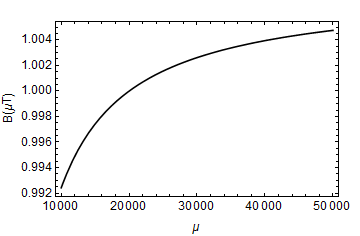
\includegraphics[width=0.6\textwidth]{B_vs_mu.png}
    \caption{caption}
     \vspace{-2.em}
    \label{fig:TRIUMF_UCN}
    \end{center}
\end{figure} 





\subsection{Magnetostatic Simulation Results}

%%%%%%%%%%%%%%%%%%%%%%%%%%%%%%%%%%%%%%%%%%%%%%%%%%%%%%%%%%%%%%%%%%%%55
% Jeff; need to decide graphs with Taraneh.
%%%%%%%%%%%%%%%%%%%%%%%%%%%%%%%%%%%%%%%%%%%%%%%%%%%%%%%%%%%%%%%%%%%%55
\begin{itemize}
\item I think it would be easy to provide results in axisymmetric
  geometries from FEMM.
\item If any result is available from OPERA, it could be included here.
\item Results should be for a restricted set of possible nEDM coils.
\item quote reaction factors?
\item One graph?  % probably the same graph as above
\end{itemize}

\subsection{Self-Shielded Coils}

%%%%%%%%%%%%%%%%%%%%%%%%%%%%%%%%%%%%%%%%%%%%%%%%%%%%%%%%%%%%%%%%%%%%55
% Chris B advises to make this section much more vague and shorter.
% (Jeff can do)
%%%%%%%%%%%%%%%%%%%%%%%%%%%%%%%%%%%%%%%%%%%%%%%%%%%%%%%%%%%%%%%%%%%%55
\begin{itemize}
\item Explain principle (reaction factor = 1, or no field at shield so
  no return flux)
\item Simple analytic results - reaction factor is identically unity.
\item FEMM/OPERA - demonstrate that sensitivity is reduced by factor
  of XX for simple geometry.
\item One graph, or include on previous graph?
\end{itemize}

\subsection{Summary of $B_0(\mu)$}

%%%%%%%%%%%%%%%%%%%%%%%%%%%%%%%%%%%%%%%%%%%%%%%%%%%%%%%%%%%%%%%%%%%%55
% Taraneh
%%%%%%%%%%%%%%%%%%%%%%%%%%%%%%%%%%%%%%%%%%%%%%%%%%%%%%%%%%%%%%%%%%%%55
Insert summary here.

\section{Measurements of $\mu(T)$}

\subsection{Previous Measurements and their Relationship to nEDM Experiments}

\begin{itemize}
\item Coucheron et al.?
\item Krupp-VDM data sheet?
\item Proper literature search on past measurements of $\mu(T)$.
\item State caveats in order to use these:  dependence on B, H, f.
\item State typical B, H, f that nEDM needs.  Motivates additional
  measurements.
\end{itemize}

\subsection{Axial Shielding Factor Measurements}

\begin{itemize}
\item Describe experimental setup and important considerations
  (e.g. relationship of data to effective $\mu$)
\item Explain B, H, f, and dominant systematic effects.
\item One figure of experimental setup?
\item One data graph?
\item State overall result and systematic error.
\end{itemize}

\subsection{Transformer Core Measurements}

\begin{itemize}
\item Describe experimental setup and important consdierations (e.g. relationship of data to effective $\mu$)
\item Explain B, H, f, and dominant systematic effects.
\item Understanding in terms of Jiles-Atherton.  Complications that
  this does not translate well into ``$\mu$''.
\item One data graph?  (Perhaps the Jiles-Atherton one?)
\item State overall result and systematic error.
\end{itemize}
%%%%%%%%%%%%%%%%%%%%%%%%%%%%%%%%%%%%%%%%%%%%%%%%%%%%%%%%%%%%%%%%%%%%%%
% Taraneh, can you write text up to this point?
%%%%%%%%%%%%%%%%%%%%%%%%%%%%%%%%%%%%%%%%%%%%%%%%%%%%%%%%%%%%%%%%%%%%%%

\subsection{Summary of $\mu(T)$}

Insert Summary Here.

\section{Summary and Conclusions}

\begin{itemize}
\item We determined $dB_0/d\mu$.  For reasonable parameters its $\sim$ XXX.  For self-shielded it's reduced by a factor of XXX for realistic windings.
\item We measured $d\mu/dT$.  We constrained it to be in the range 0.1
  to 2.3 percent per Kelvin.  Dominant errors are XXX for each method.
  Neither method is for correct B, H, f.  Both methods are very
  difficult to achieve consistent sub-percent determinations, but tend
  to agree on sign and magnitude of problem.
\item Results imply temperature stability to XXX Kelvin for stability
  goal of XXX pT.  Show that this could be a dominant issue for
  stability for future experiments.  Not addressed by many other
  measurements which tend to focus on stability at zero field or
  overall stability in full EDM experiment.
\item Future work: build full EDM experiment.  Capability of various
  internal coil geometries and best achievable temperature stability
  are both important to success.
\end{itemize}

\section{To Do List}

\begin{enumerate}
\item Collect graphs and figures.
\begin{enumerate}
\item Analytical comparison reaction factor vs. $\mu$ for
  sphere and/or cylinder with reasonable geometry/$\mu$.
\item Same or additional comparison for more realistic geometry in
  simulation.  May include self-shielded geometry.
\item Axial shielding factor figure of setup.
\item Axial shielding factor data.
\item Transformer core Jiles-Atherton comparison?
\end{enumerate}
\item Write.
\end{enumerate}

\section*{References}

\bibliography{mybibfile}
\begin{thebibliography}{00}

\bibitem{bib:nedm1} S. N. Balashov {\it et al.}, arXiv:0709.2428.

\bibitem{bib:nedm2} A. P. Serebrov {\it et al.}, JETP Lett. {\bf 99}, 4
  (2014).

\bibitem{bib:nedm2.5} A. P. Serebrov {\it et al.}, Physics Procedia {\bf
  17}, 251 (2011).

\bibitem{bib:nedm3} K. Kirch, AIP Conf. Proc., Vol. 1560, pp. 90-94
  (2013).

\bibitem{bib:nedm3.5} C. A. Baker, {\it et al.}, Physics Procedia {\bf
  17}, 159 (2011).

\bibitem{bib:nedm4} Y. Masuda, K. Asahi, K. Hatanaka, S.-C. Jeong,
  S. Kawasaki, R. Matsumiya, K. Matsuta, M. Mihara, and Y. Watanabe,
  Phys. Lett. A {\bf 376}, 1347 (2012).

\bibitem{bib:nedm5} I. Altarev, {\it et al.}, Nuovo Cim. C {\bf
  35}, 122 (2012).

\bibitem{bib:nedm6} R. Golub and S. K. Lamoreaux, Phys. Rept.  {\bf
  237}, 1 (1994).

\bibitem{bib:nedm6.5} T. M. Ito (the nEDM collaboration),
  J. Phys. Conf. Ser. {\bf 69} 012037, 2007.

\bibitem{bib:baker} C. A. Baker, {\it et al.}, Phys. Rev. Lett. {\bf
  97}, 131801 (2006).

\bibitem{bib:brys} T. Bry\'s, {\it et al.}, Nucl. Instrum. Meth. A
  {\bf 554}, 527 (2005).

\bibitem{bib:afach} S. Afach, {\it et al.}, J. Appl. Phys. 116, 084510 (2014).

\bibitem{bib:fierlingerroom} I. Altarev, {\it et al.}
  Rev. Sci. Instrum. {\bf 85}, 075106 (2014).

\bibitem{bib:sturmthesis} M. Sturm, Masterarbeit, T.U. Muenchen (2013).

\bibitem{bib:patton} B. Patton, E. Zhivun, D. C. Hovde, and D. Budker,
  Phys. Rev. Lett. 113, 013001 (2014).
\bibitem{bib:couderchon} G. Couderchon, J. F. Tiers, J. Magn. Magn. Mat. 26(1):196-214 (1982).

\bibitem{bib:bidinosti} C. P. Bidinosti, AIP Advances 4, 047135 (2014).

\bibitem{bib:smythe} W. R. Smythe, McGraw Hill (1950).

\bibitem{bib:ferraro} V. C. A. Ferraro, Athalone Press (1967).

\bibitem{bib:gupta} Kiran Gupta, K. K. Raina, S. K. Sinha, J. Alloys Compd, 429(1):357-364 (2007).
\end{thebibliography}

\end{document}
